% Created 2021-04-21 Wed 21:00
% Intended LaTeX compiler: xelatex
\documentclass[12pt]{article}
\usepackage{graphicx}
\usepackage{grffile}
\usepackage{longtable}
\usepackage{wrapfig}
\usepackage{rotating}
\usepackage[normalem]{ulem}
\usepackage{amsmath}
\usepackage{textcomp}
\usepackage{amssymb}
\usepackage{capt-of}
\usepackage{hyperref}
\usepackage{minted}
\usepackage{amsmath}
\usepackage{amssymb}
\usepackage{setspace}
\usepackage{subcaption}
\usepackage{mathtools}
\usepackage{xfrac}
\usepackage[margin=1in]{geometry}
\usepackage{marginnote}
\usepackage[utf8]{inputenc}
\usepackage{color}
\usepackage{epsf}
\usepackage{tikz}
\usepackage{graphicx}
\usepackage{pslatex}
\usepackage{hyperref}

\usepackage{beton}
\usepackage{euler}
\usepackage[OT1]{fontenc}

\usepackage{textgreek}
\renewcommand*{\textgreekfontmap}{%
{phv/*/*}{LGR/neohellenic/*/*}%
{*/b/n}{LGR/artemisia/b/n}%
{*/bx/n}{LGR/artemisia/bx/n}%
{*/*/n}{LGR/artemisia/m/n}%
{*/b/it}{LGR/artemisia/b/it}%
{*/bx/it}{LGR/artemisia/bx/it}%
{*/*/it}{LGR/artemisia/m/it}%
{*/b/sl}{LGR/artemisia/b/sl}%
{*/bx/sl}{LGR/artemisia/bx/sl}%
{*/*/sl}{LGR/artemisia/m/sl}%
{*/*/sc}{LGR/artemisia/m/sc}%
{*/*/sco}{LGR/artemisia/m/sco}%
}
\makeatletter
\newcommand*{\rom}[1]{\expandafter\@slowromancap\romannumeral #1@}
\makeatother
\DeclarePairedDelimiterX{\infdivx}[2]{(}{)}{%
#1\;\delimsize\|\;#2%
}
\newcommand{\infdiv}{D\infdivx}
\DeclarePairedDelimiter{\norm}{\left\lVert}{\right\rVert}
\DeclarePairedDelimiter{\ceil}{\left\lceil}{\right\rceil}
\DeclarePairedDelimiter{\floor}{\left\lfloor}{\right\rfloor}
\def\Z{\mathbb Z}
\def\R{\mathbb R}
\def\C{\mathbb C}
\def\N{\mathbb N}
\def\Q{\mathbb Q}
\def\noi{\noindent}
\onehalfspace
\usemintedstyle{bw}
\author{Sandy Urazayev\thanks{University of Kansas (ctu@ku.edu)}}
\date{44; 12021 H.E.}
\title{Homework 1 Oracle\\\medskip
\large MATH 220 Spring 2021}
\hypersetup{
 pdfauthor={Sandy Urazayev},
 pdftitle={Homework 1 Oracle},
 pdfkeywords={},
 pdfsubject={},
 pdfcreator={Emacs 28.0.50 (Org mode 9.4.5)}, 
 pdflang={English}}
\begin{document}

\maketitle
\href{./index.pdf}{View the PDF version​}

\section*{Chapter 1.1}
\label{sec:org8c1fbcd}
\subsection*{Problem 7}
\label{sec:org70a5c8b}
\begin{center}
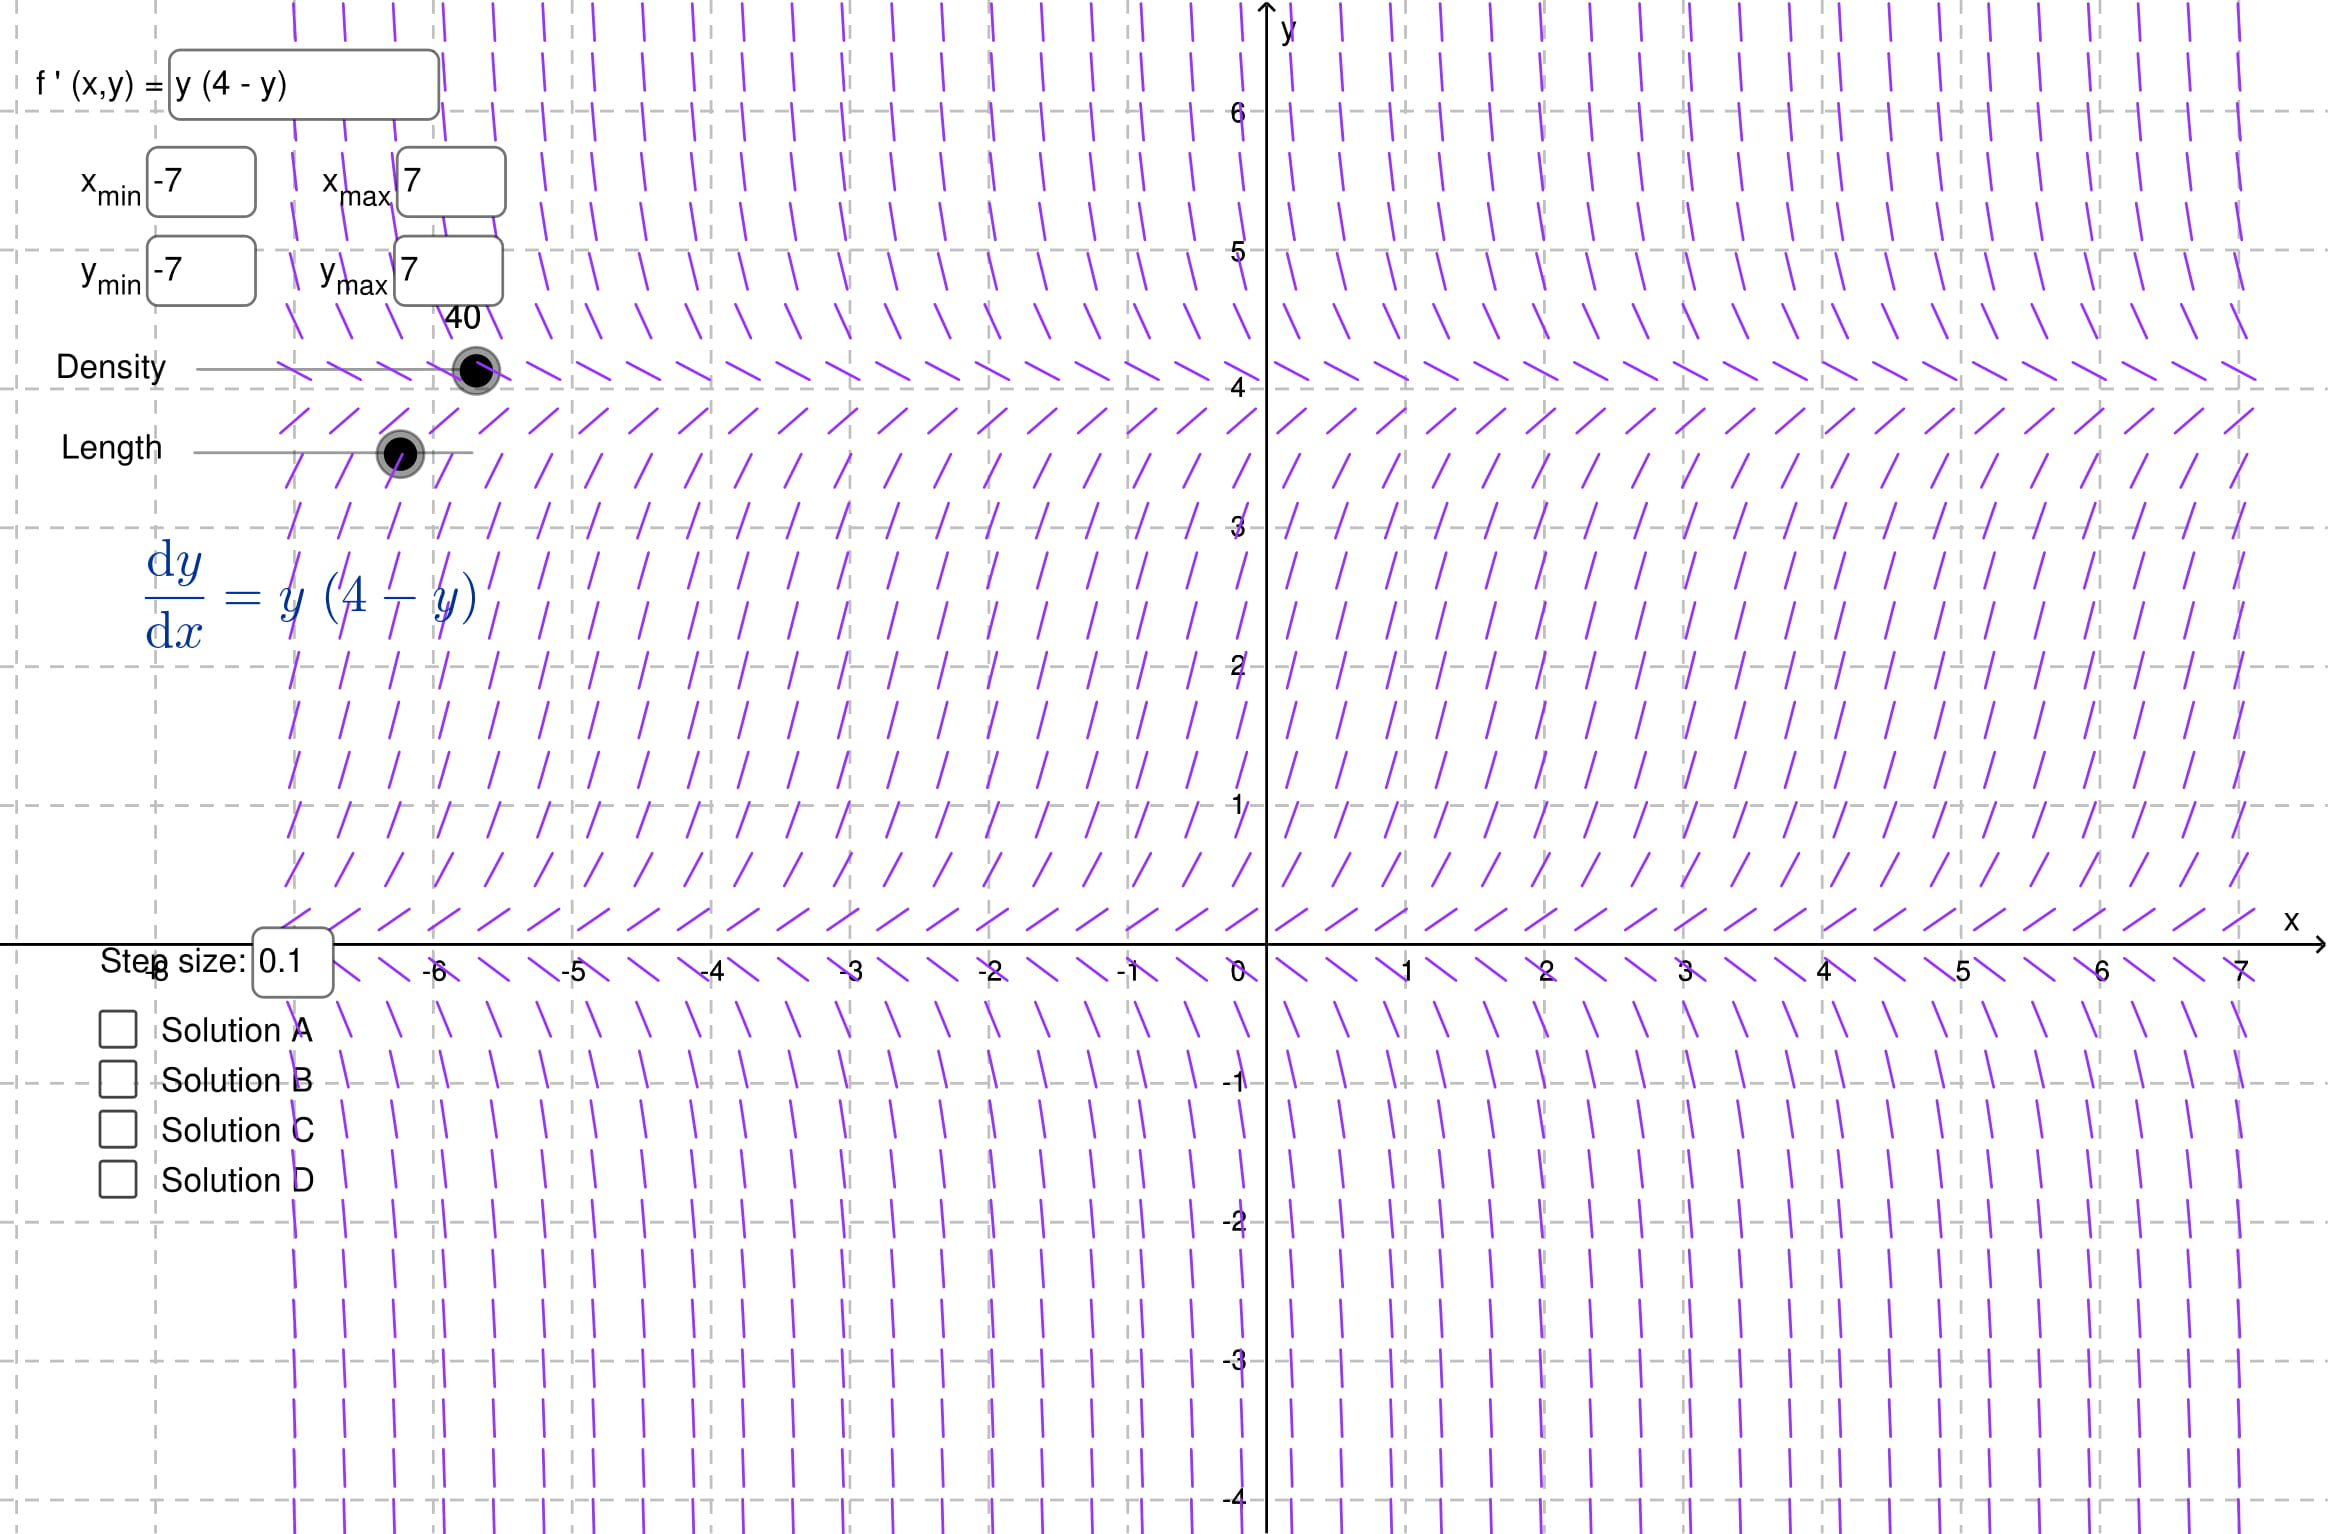
\includegraphics[width=.9\linewidth]{./7.jpg}
\end{center}
\subsection*{Problem 10}
\label{sec:orgffbd5f5}
\begin{center}
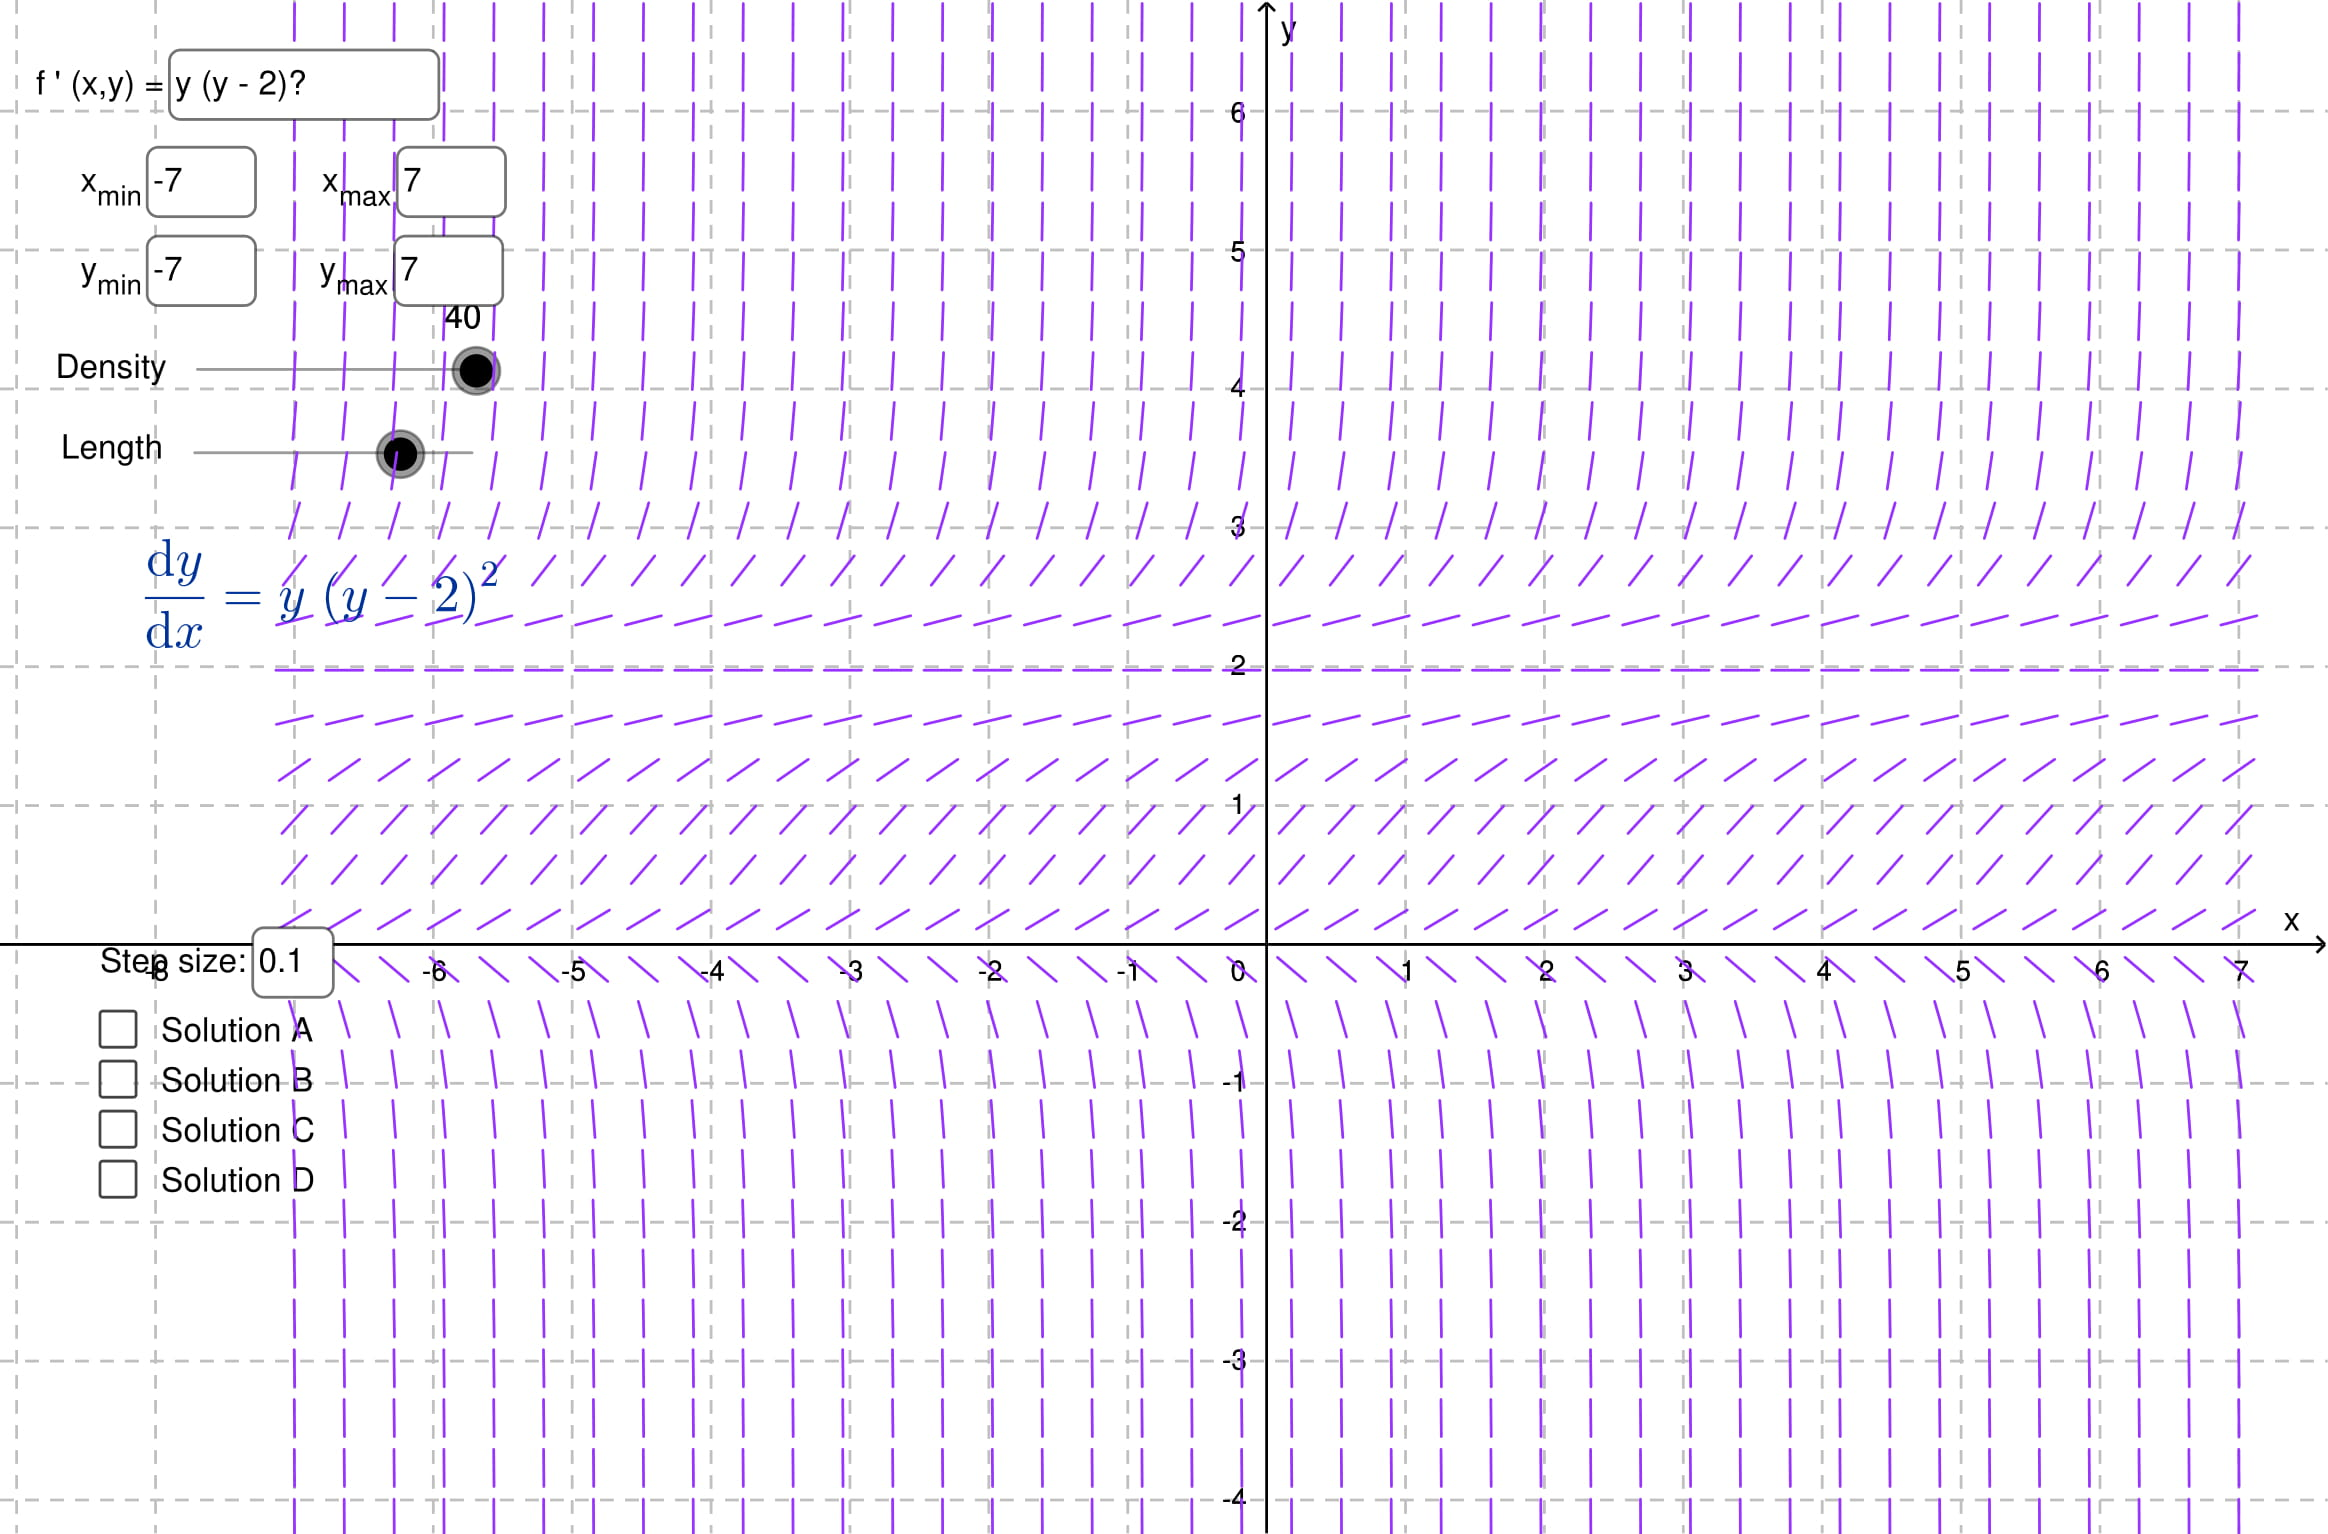
\includegraphics[width=.9\linewidth]{./10.jpg}
\end{center}
\subsection*{Problem 15 [FOR GRADE]}
\label{sec:orgd5ed1ad}
We can see that the direction field results in constant rate of change of
zero at level where \(y=0\) and \(y=3\). Then we can also see that the direction
of the graph decreases when \(y<0\) and \(y>3\), while also increasing in section
of \(y>0\) and \(y<3\). That means, we are looking for a separate \(y\) to get
constant change at \(0\) and \((3-y)\) term, so that the constraints above are
satisfied. \(\therefore y' = y(3-y)\). Answer is \texttt{h}.
\section*{Chapter 1.2}
\label{sec:orga6fb566}
\subsection*{Problem 7 [FOR GRADE]}
\label{sec:org11544b4}
Our differential equation is as given
\begin{equation*}
        \frac{dp}{dt} = \frac{p}{2} - 450
\end{equation*}

\textbf{a}. Find the time at which the population becomes extinct if \(p(0)=850\)

We find that \(\mu(t) = e^{\int -\frac{1}{2} dt} = e^{-\frac{1}{2}t}\). Then

\begin{align*}
        \frac{d}{dt}(\mu(t)p) = -450 \mu(t)                                                 \\
        \implies p(t) & = \frac{\int -450\mu(t) dt}{\mu(t)}                                 \\
                      & = \frac{\int -450 e^{-\frac{1}{2}t}dt}{e^{-\frac{1}{2}t}}         \\
                      & = \frac{-450 \times (-2e^{-\frac{1}{2}t}) + C}{e^{-\frac{1}{2}t}} \\
                      & = 900 + C e^{\frac{1}{2}t}
\end{align*}

Then by using \(p(0)=850\), we find the constant \(C\) to be \(-50\). We need to
find the time \(t_e\), at which \(p(t_e)=0\). We simply solve the equation
\(0 = 900 - 50 e^{\frac{1}{2}t_e}\), where we find \(t_e = \ln(324) \approx 5.78\). 

\textbf{b.} Find the time of extinction if \(p(0)=p_0\), where \(0<p_0<900\)

Using the above, we find that \(t_e = 2 \ln(\frac{900}{900-p_0})\)

\textbf{c.} Find the initial population \(p_0\) if the population is to become extinct in
1 year.

Recall from Example 1 that \(t\) is measured in months. So we simply solve
\begin{equation*}
        0 = 900 - (900-p_0)e^{6} \implies p_0 = 900 - \frac{900}{e^6} \approx 897.77
\end{equation*}
\subsection*{Problem 9}
\label{sec:orgd3bb4f6}
\textbf{a.} If the limiting velocity is 49m/s (the same as in Example 2), show that
 the equation of motion can be written as
\begin{equation*}
  \frac{dv}{dt} = \frac{1}{245}(49^2-v^2)
\end{equation*}

Recall the base equation from Example 2, by using the given, we have
\begin{equation*}
  0 = 9.8 - C (49^2) \implies C = \frac{9.8}{49^2} = \frac{1}{245}\\
  \implies \frac{dv}{dt} = \frac{1}{245}(49^2-v^2)
\end{equation*}

\textbf{b.} If \(v(0) = 0\), find an expression for \(v(t)\) at any time.

We can view this problem as a first-order separable equation and rewrite it
as
\begin{equation*}
        \int{\frac{dv}{49^2-v^2}} = \int{\frac{dt}{245}}
\end{equation*}
After some computations, the expression for \(v(t)\) is
\(49\tanh(\frac{t}{5})\)

\textbf{c.} Plot your solution from part b and the solution (26) from Example 2 on
the same axes.

\begin{center}
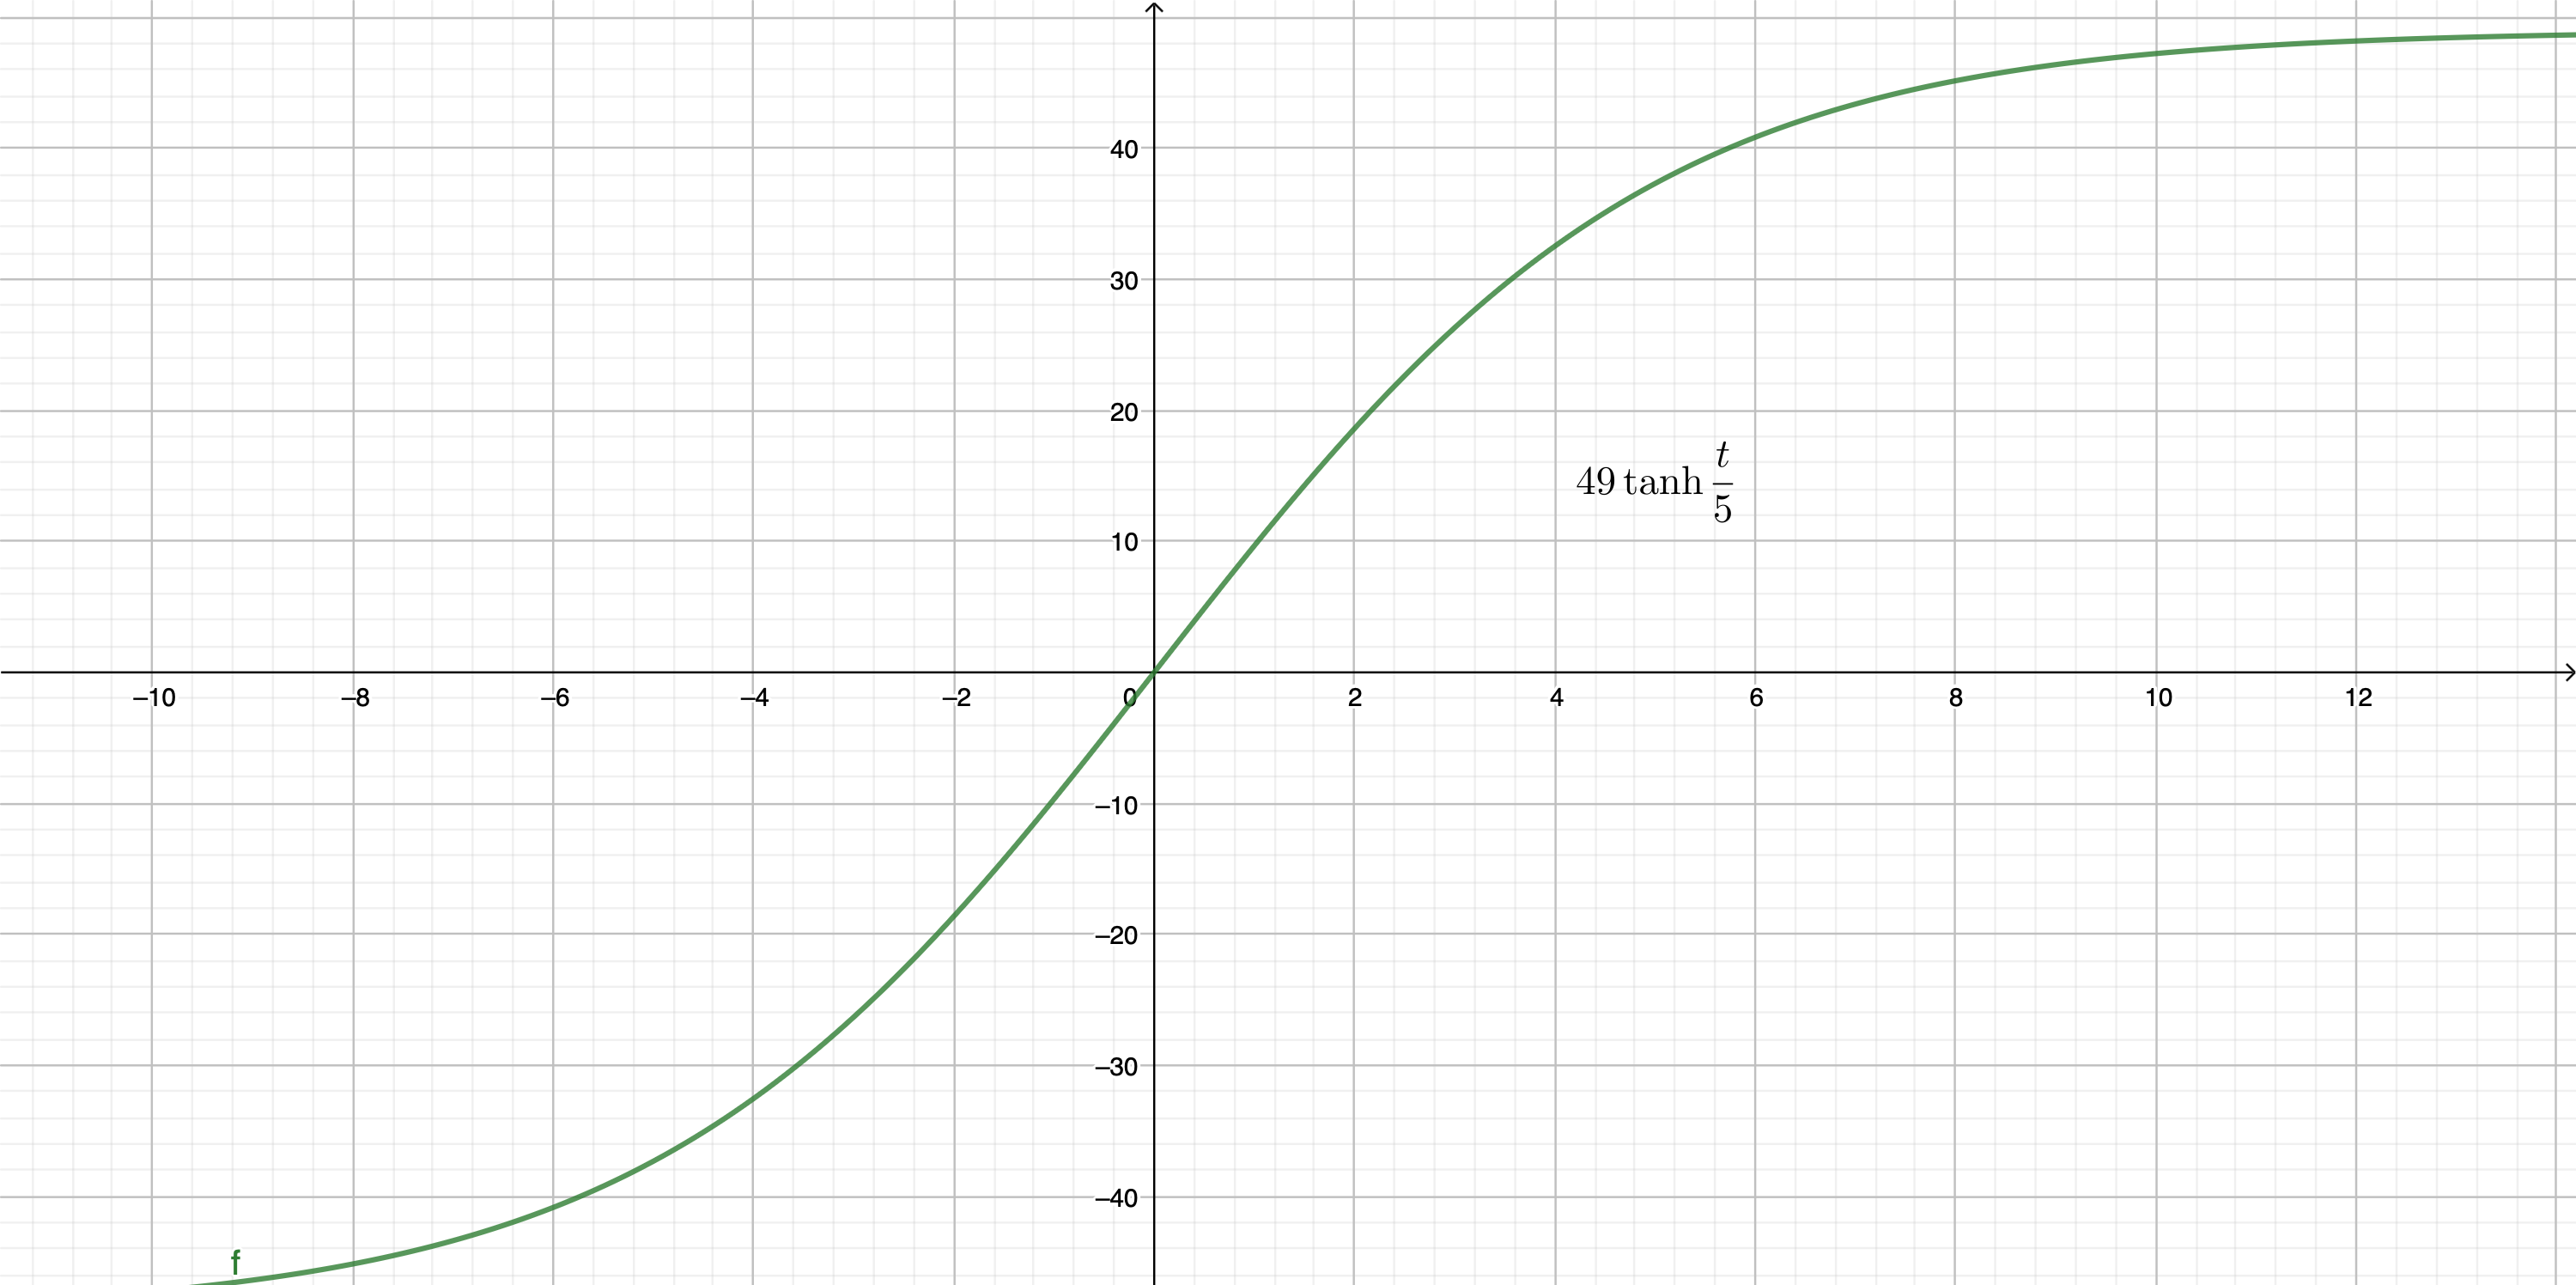
\includegraphics[width=.9\linewidth]{./tanh.png}
\end{center}

\textbf{d.} Based on your plots in part \textbf{c}, compare the effect of a quadratic drag
force with that of a linear drag force. 

The quadratic drag damps the speed faster and has a bigger effect on the
speed than the linear dependance.

\textbf{e.} Find the distance \(x(t)\) that the object falls in time \(t\).

We know that \(\frac{dx}{dt} = v(t) = 49\tanh(\frac{t}{5})\) so then
\(x(t) = 245\ln(\cosh(\frac{t}{5})) + C\). If \(x(0) = 0\), then \(C = 0\).

\textbf{f.} Find the time \(T\) it takes the object to fall 300m.

Simply solve \(300 = 245 \ln(\cosh(\frac{t}{5}))\), it will be something like
    \(t = 5\cosh^{-1}(e^{\frac{60}{49}}) \approx 9.477\)

\section*{Chapter 1.3}
\label{sec:org8235204}
\subsection*{Problem 1}
\label{sec:org1a7c332}
2nd order and linear.
\subsection*{Problem 3}
\label{sec:org6228274}
4th order and linear.
\subsection*{Problem 5}
\label{sec:orgc66051a}
Plug them both in. They are solutions.
\subsection*{Problem 9}
\label{sec:orgfddf949}
Plug them both in. They are solutions.
\subsection*{Problem 11 [FOR GRADE]}
\label{sec:org10d5088}
\(y'+2y=0\) form yields solutions for \(r=-2\). You can solve a characteristic
polynomial of this equation to get it.
\emph{I guess you guys aren't ready for that yet. But your kids are gonna love it}

\subsection*{Problem 16}
\label{sec:orgd1a5b08}
\(u_{xx} + u_{yy} + u_{zz} = 0\) is linear and second order.  

\subsection*{Problem 20}
\label{sec:org4e73e15}
Plug them both in. They are solutions.
\end{document}